\chapter{Force-Guided Robot Alignment}
\label{chapter4}
\hspace*{6mm}In this chapter, an Forces and Torques (F/T) sensor is involved and force-guided robot alignment is proposed. Problem definition is addressed in section \ref{sec:pro def} followed by Integration of F/T sensor in senction \ref{sec:grav compen}. Admittance control based on F/T sensor is described in section \ref{sec:adm ctrl}. Coordinate transformation of F/T sensor will is interpreted in section \ref{sec:rfc}. Parameter selection of  admittance control is discussed in section \ref{sec:affection}.
\section{Problem Definition and Proposed Method}
\label{sec:pro def}
\hspace*{6mm}In this section, problem definition is addressed followed by a brief introduction of proposed method.
\subsubsection{Problem Definition}
\hspace*{6mm}In modern robot-assisted surgery, to simulate the eyes of doctors,  image processing is often considered. With the image's information, the surgeon can obtain real-time data that humans can not observe clearly. Surgeons use the image process to do many things, such as tracking whether the patient is moving, positioning an incision point, and navigating an insertion path. As for root canal treatment, the endodontist checks the number of root canals with computed tomography.  Before starting to clean the pulp, the endodontist tries to insert root files into root canals. Then the endodontist takes the patient to have computed tomography(CT). CT scan can clearly show the tooth with the root files. With the preoperative image, the endodontist can check whether all root canals are all found and determine all root canals' lengths. However, the above image application is preoperative. The endodontist can only use the preoperative image to guess the direction of the insertion. The intraoperative image processing is absent due to the dimension restriction of a tooth. It is difficult to get a real-time image when the dentist inserts a root file into the opened tooth because it will obstacle the observation. Besides, the diameter of a root canal is $1$ mm and is smaller than a root file. It is impossible to get the image from any shooting angle.
\subsubsection{Proposed Method}
\hspace*{6mm}To solve the first problem -- without image processing, admittance control based on F/T sensor is reviewed. The literature on peg-in-hole based on F/T sensor  \cite{7743375, pihwithflex, Xu201511, 8294275} are surveyed because the cleaning procedure is similar to it. To apply in different situation, two operating modes -- "Dragging Mode" and "Self-Alignment Mode" are designed. In "Dragging Mode", Dentists can hold the handpiece to the desired position and orientation. In "Self-Alignment Mode", the handpiece can automatically align the root canal direction with any complicated conditions. Two modes are set by change reference frame and parameter setting.
\section{Integration of F/T sensor}
\label{sec:grav compen}
\hspace*{6mm}In this section, technical solution to system integration with an F/T sensor is discuused. In Figure \ref{fig:gravity compensation} shows that initial value and gravity load affect the value of F/T sensor. Hence, gravity compensation and initial value are compensated and discussed followd by external force evaluation.
\begin{figure}[htbp]
\begin{center}
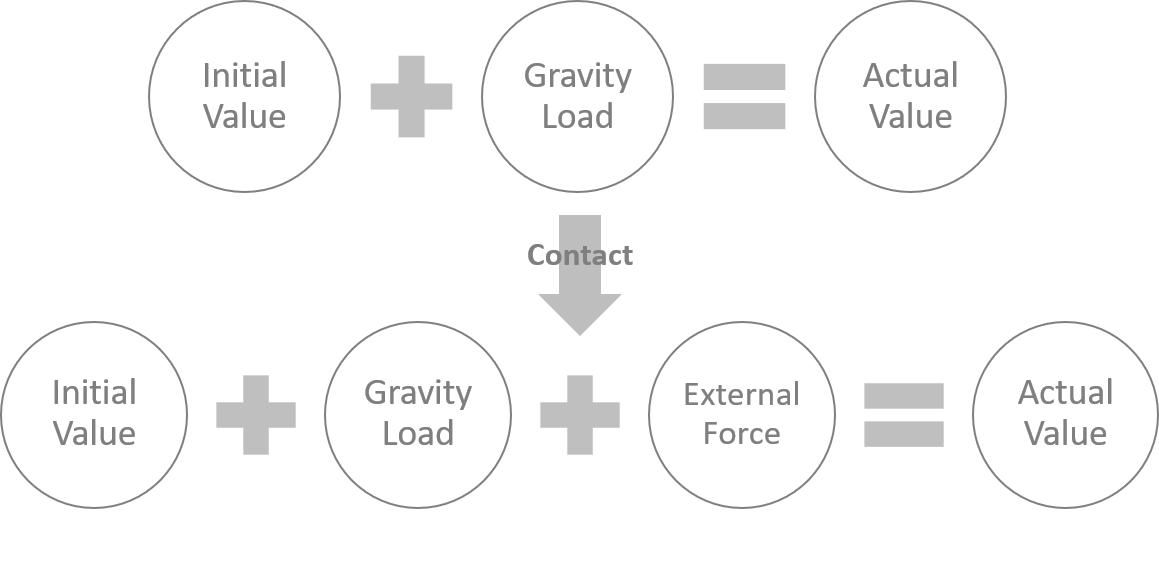
\includegraphics[width=1\linewidth]{Images/gravity compensation.png}
\caption{
Data analysis of F/T sensor.
}\label{fig:gravity compensation}
\end{center}
\end{figure}
\subsubsection{Gravity Compensation and Initial Value Reset}
\hspace*{6mm}Gravity compensation is a critical technical issue when combining an F/T sensor with a robot arm and an end effector \cite{8997006}. 
Fundamentally, we should receive stable data when a static F/T sensor bears the same load or force. Nevertheless, our F/T sensor is installed on the robot arm and move with the pose of the robot arm. On account of its mobility, the gravity of the end effector will significantly affect the actual value we received. Moreover, starting without resetting the F/T sensor to zero would lead to an initial value. If we could not analyze the actual value to an initial value and a gravity load, we would obtain an unstable actual value, not to mention the external force caused by contact force. Therefore, we illustrate a method, which is to analyze the actual value of the F/T sensor to an initial value and gravity load in real-time. It's worth noting that with this approach, we can get the installation angle between the F/T sensor and the robot arm, including assembly error, and we no longer need to reset the F/T sensor to zero every time.
\par
The actual value measured by F/T sensor is expressed as [$f_{x}$ $f_{y}$ $f_{z}$ $\tau_{x}$ $\tau_{y}$ $\tau_{z}$], which is affected by initial value expressed as [$f_{0x}$ $f_{0y}$ $f_{0z}$ $\tau_{0x}$ $\tau_{0y}$ $\tau_{0z}$] and gravity load expressed as [$f_{gx}$ $f_{gy}$ $f_{gz}$ $\tau_{gx}$ $\tau_{gy}$ $\tau_{gz}$]. Initial value is the value without resetting F/T sensor and gravity load is the gravity of the end effector.
\begin{equation}\label{eq:gc_iga}
\begin{split}
\text{Actual Value} &= \text{Initial value}	+ \text{Gravity Load}\\
\boldsymbol{f} 		&= 	\boldsymbol{f_0}		+\boldsymbol{f_g}	\\ 
\boldsymbol{\tau}	&=	\boldsymbol{\tau_0}		+\boldsymbol{\tau_g}
\end{split}
\end{equation}
where 
\begin{equation*}
\begin{split}
\boldsymbol{f} = 
\begin{bmatrix}
f_{x}	\\
f_{y}	\\
f_{z}
\end{bmatrix},\ 
\boldsymbol{f_0} = 
\begin{bmatrix}
f_{0x}	\\
f_{0y}	\\
f_{0z}
\end{bmatrix},\ 
\boldsymbol{f_g} = 
\begin{bmatrix}
f_{gx}	\\
f_{gy}	\\
f_{gz}
\end{bmatrix}\\
\boldsymbol{\tau} = 
\begin{bmatrix}
\tau_{x}		\\
\tau_{y}		\\
\tau_{z}	
\end{bmatrix},\ 
\boldsymbol{\tau_0} = 
\begin{bmatrix}
\tau_{0x}		\\
\tau_{0y}		\\
\tau_{0z}	
\end{bmatrix},\ 
\boldsymbol{\tau_g} = 
\begin{bmatrix}
\tau_{gx}		\\
\tau_{gy}		\\
\tau_{gz}	
\end{bmatrix}
\end{split}
\end{equation*}
\par\noindent
And, by terms of moment arm formula,
\begin{equation}
\label{eq:moment arm}
\begin{split}
\boldsymbol{\tau_g}	&= \boldsymbol{r} \times \boldsymbol{f_g} \\
\end{split}
\end{equation}
where $\boldsymbol{r}$ denotes the centroid position of the end effector in the sensor frame.
\par\noindent
Combines Equation \ref{eq:gc_iga} and Equation \ref{eq:moment arm},
\begin{equation}
\label{eq: middle}
\begin{split}
\boldsymbol{\tau}	&=	\boldsymbol{\tau_0}		+\boldsymbol{\tau_g}			\\
					&= 	\boldsymbol{\tau_0}	 	+\boldsymbol{r} \times \boldsymbol{f_g}	\\
					&=  \boldsymbol{\tau_0}		+\boldsymbol{r}	\times \left( \boldsymbol{f} - \boldsymbol{f_0} \right) 
\end{split}
\end{equation}
Equation \ref{eq: middle} can be extend as 
\begin{equation}
\begin{split}
\tau _{x}	&=	\tau _{0x} 	+ \left( f_z - f_{0z}\right) \cdot y - \left( f_y - f_{0y}\right) \cdot z\\
\tau _{y}	&=	\tau _{0y}	+ \left( f_x - f_{0x}\right) \cdot z - \left( f_z - f_{0z}\right) \cdot x\\
\tau _{z}	&=	\tau _{0z}	+ \left( f_y - f_{0y}\right) \cdot x - \left( f_x - f_{0x}\right) \cdot y 
\end{split}
\end{equation}
and be overwritten as
\begin{equation}\label{eq:matrix_mfrk}
\begin{split}
\begin{bmatrix}
\tau _x\\
\tau _y\\
\tau _z
\end{bmatrix}
=
\begin{bmatrix}
0		&f_z	&-f_y	&1	&0	&0\\
-f_z	&0		&f_x	&0	&1	&0\\
f_y		&-f_x	&0		&0	&0	&1
\end{bmatrix}
\begin{bmatrix}
x\\
y\\
z\\
k_1\\
k_2\\
k_3
\end{bmatrix}\\
\end{split}
\end{equation}
\par\noindent
where $k_1$, $k_2$, $k_3$ are all constants and
\begin{equation}\label{eq:k1k2k3}
\begin{split}
k_1 = \tau _{0x} - \left( f_{0z} \cdot y + f_{0y} \cdot z \right)  \\
k_2 = \tau _{0y} - \left( f_{0x} \cdot z + f_{0z} \cdot x \right)  \\
k_3 = \tau _{0z} - \left( f_{0y} \cdot x + f_{0x} \cdot y \right)  
\end{split}
\end{equation}
To extract [$x$, $y$, $z$, $k_1$, $k_2$, $k_3$], we move the robot arm to $n\ (n\geq3)$ positions with different poses. By recording $n$ torque vectors and corresponding $n$ force vectors from F/T sensor, we can expand Equation \ref{eq:matrix_mfrk} as
\begin{equation}
\begin{split}
\begin{bmatrix}
\tau _x^1	\\
\tau _y^1	\\
\tau _z^1	\\
\tau _x^2	\\
\tau _y^2	\\
\tau _z^2	\\
\vdots\\
\tau _x^n	\\
\tau _y^n	\\
\tau _z^n	
\end{bmatrix}
=
\begin{bmatrix}
0			&f_z^1		&-f_y^1		&1	&0	&0\\
-f_z^1		&0			&f_x^1		&0	&1	&0\\
f_y^1		&-f_x^1		&0			&0	&0	&1\\
0			&f_z^2		&-f_y^2		&1	&0	&0\\
-f_z^2		&0			&f_x^2		&0	&1	&0\\
f_y^2		&-f_x^2		&0			&0	&0	&1\\
 			& 			&\vdots		& 	& 	& \\
0			&f_z^3		&-f_y^3		&1	&0	&0\\
-f_z^3		&0			&f_x^3		&0	&1	&0\\
f_y^3		&-f_x^3		&0			&0	&0	&1
\end{bmatrix}
\begin{bmatrix}
x\\
y\\
z\\
k_1\\
k_2\\
k_3
\end{bmatrix}\\
\end{split}
\end{equation}
which is defined as 
\begin{equation*}
\begin{split}
\boldsymbol{m}_{\left(3n \times 1\right)} = \mathbf{F}_{\left(3n \times 6\right)} \cdot \boldsymbol{p}_{\left(6 \times 1\right)}
\end{split}
\end{equation*}
Due to the full column rank of $\mathbf{F}$, we can apply Moore-Penrose pseudoinverse. Then, 
\begin{equation*}
\begin{split}
\boldsymbol{p} 	&= \mathbf{F}^{\dagger} \cdot \boldsymbol{m}\\
				&= \left( \mathbf{F}^\top\mathbf{F}\right) ^{-1}\mathbf{F}^\top \cdot \boldsymbol{m}
\end{split}
\end{equation*}
\par
So far, we have obtained a middle information [$x$ $y$ $z$ $k_1$ $k_2$ $k_3$]. Note that [$x$ $y$ $z$] is the centroid position of end effector related to the sensor frame. [$k_1$ $k_2$ $k_3$] is still coupled by initial forces [$f_{0x}$ $f_{0y}$ $f_{0z}$] and torque values [$\tau_{0x}$ $\tau_{0y}$ $\tau_{0z}$].
\par
To decouple [$k_1$ $k_2$ $k_3$], let us return to the first equation in Figure \ref{fig:gravity compensation}. We continue to use this formula and contemplate it from the perspective of coordinate transformation relation. Here we hypothesize that the end effector weighs $g$ kilograms relative to the frame\{0\} which is also the world frame. That means the gravity vector of the end effector $^{\{0\}}\boldsymbol{g}$ is [$0$ $0$ $-g$] related to the frame\{0\}. Then,
\begin{equation}
\label{eq:ffrrg}
\begin{split}
\text{Actual Value} &= \text{Initial value}	+ \text{Gravity Load}\\
\Rightarrow
\boldsymbol{f}		&= \boldsymbol{f_0} +\boldsymbol{f_g}\\
					&= \boldsymbol{f_0} +\ ^\mathrm{S}_6\mathbf{R} \cdot ^6_0\!\mathbf{R} \cdot \boldsymbol{^0\!g}
\end{split}
\end{equation}
\par\noindent
which is relative to frame \{6\}.
Hence, we assume an installation angle $\theta$ including assembly error.
\begin{equation}
\begin{split}
 ^\mathrm{S}_6\mathbf{R}
=
\begin{bmatrix}
\cos(\theta)	&\sin(\theta)	&0 \\
-\sin(\theta)	&\cos(\theta)	&0 \\
0				&0				&1
\end{bmatrix}
\end{split}
\end{equation}
Besides, we can easily calculate $^6_0\mathbf{R}$ from Equation \ref{eq:translation matrix}.
\begin{equation}
\begin{split}
^6_0\mathbf{R} 	&=\ ^0_6\mathbf{R}^\top\\
				&\coloneqq
\begin{bmatrix}
r_{11}		&r_{12}		&r_{13} \\
r_{21}		&r_{22}		&r_{23} \\
r_{31}		&r_{32}		&r_{33}
\end{bmatrix}
\end{split}
\end{equation}
Therefore,
\begin{equation}
\label{eq:frrgf}
\begin{split}
\begin{bmatrix}
f_{0x}\\
f_{0y}\\
f_{0z}
\end{bmatrix}
+
\begin{bmatrix}
\cos(\theta)	&\sin(\theta)	&0 \\
-\sin(\theta)	&\cos(\theta)	&0 \\
0				&0				&1
\end{bmatrix}
\begin{bmatrix}
r_{11}		&r_{12}		&r_{13} \\
r_{21}		&r_{22}		&r_{23} \\
r_{31}		&r_{32}		&r_{33}
\end{bmatrix}
\begin{bmatrix}
0\\
0\\
-g
\end{bmatrix}
=
\begin{bmatrix}
f_x\\
f_y\\
f_z
\end{bmatrix}
\end{split}
\end{equation}
Equation \ref{{eq:frrgf}} can be rewritten as 
\begin{equation}
\label{eq:matrix_rgf0f}
\begin{split}
\begin{bmatrix}
-r_{13}		&-r_{23} 	&0			&1		&0		&0\\
-r_{23}		&r_{13}		&0			&0		&1		&0\\
0			&0			&-r_{33}	&0		&0		&1
\end{bmatrix}
\begin{bmatrix}
g\cos(\theta)\\
g\sin(\theta)\\
g\\
f_{0x}\\
f_{0y}\\
f_{0z}
\end{bmatrix}
=
\begin{bmatrix}
f_x\\
f_y\\
f_z
\end{bmatrix}
\end{split}
\end{equation}
To extract $[g\cos(\theta),g\sin(\theta),g,f_{0x},f_{0y},f_{0z}]$ with the least square solution, $n(n\geq3)$ third columns of ration matrices and corresponding $n$ force vectors from F/T sensor are recorded in real-time. Therefore, Equation \ref{eq:matrix_rgf0f} can be expended as
\begin{equation}
\begin{split}
\begin{bmatrix}
-r_{13}^1		&-r_{23} ^1		&0			&1		&0		&0\\
-r_{23}^1		&r_{13}^1		&0			&0		&1		&0\\
0				&0				&-r_{33}^1	&0		&0		&1\\
-r_{13}^2		&-r_{23}^2 		&0			&1		&0		&0\\
-r_{23}^2		&r_{13}^2		&0			&0		&1		&0\\
0				&0				&-r_{33}^2	&0		&0		&1\\
&&\vdots\\
-r_{13}^n		&-r_{23}^n 		&0			&1		&0		&0\\
-r_{23}^n		&r_{13}^n		&0			&0		&1		&0\\
0				&0				&-r_{33}^n	&0		&0		&1
\end{bmatrix}
\begin{bmatrix}
g\cos(\theta)\\
g\sin(\theta)\\
g\\
f_{0x}\\
f_{0y}\\
f_{0z}
\end{bmatrix}
=
\begin{bmatrix}
f^1_{0x}\\
f^1_{0y}\\
f^1_{0z}\\
f^2_{0x}\\
f^2_{0y}\\
f^2_{0z}\\
\vdots\\
f^n_{0x}\\
f^n_{0y}\\
f^n_{0z}
\end{bmatrix}
\end{split}
\end{equation}
which is defined as 
\begin{equation*}
\begin{split}
\mathbf{M}_{\left(3n \times 6\right)} \cdot \boldsymbol{p}_{\left(6 \times 1\right)} = \boldsymbol{f}_{\left(3n \times 1\right)}
\end{split}
\end{equation*}
Due to the full column rank of $\mathbf{M}$, we can apply Moore-Penrose pseudoinverse. Then, 
\begin{equation*}
\begin{split}
\boldsymbol{p} 	&= \mathbf{M}^{\dagger} \cdot \boldsymbol{f}\\
				&= \left( \mathbf{M}^\top\mathbf{M}\right) ^{-1}\mathbf{M}^\top \cdot \boldsymbol{f}
\end{split}
\end{equation*}
So far, the load gravity $\boldsymbol{^0\!g}$ and the initial forces [$f_{0x}$ $f_{0y}$ $f_{0z}$] are obtained. Substitute the initial forces [$f_{0x}$ $f_{0y}$ $f_{0z}$] into Equation \ref{eq:k1k2k3}, then
\begin{equation}
\begin{split}
\tau _{0x}	=	k_1	+ \left( f_{0z} \cdot y + f_{0y} \cdot z \right) \\
\tau _{0y} 	=	k_2	+ \left( f_{0x} \cdot z + f_{0z} \cdot x \right) \\
\tau _{0z} 	=	k_3 + \left( f_{0y} \cdot x + f_{0x} \cdot y \right)
\end{split}
\end{equation}
Therefore, [$k_1$ $k_2$ $k_3$] are decoupled and the initial torque values [$\tau_{0x}$ $\tau_{0y}$ $\tau_{0z}$] are obtained. Substitute the load gravity $\boldsymbol{^0\!g}$ into Equation \ref{eq:moment arm} and Equation \ref{eq:ffrrg}, then
\begin{equation}
\begin{split}
\boldsymbol{f_g} &= \boldsymbol{f_0} +\ ^\mathrm{S}_6\mathbf{R} \cdot ^6_0\!\mathbf{R} \cdot \boldsymbol{^0\!g}	\\
\boldsymbol{\tau_g}	&= \boldsymbol{r} \times \boldsymbol{f_g} 
\end{split}
\end{equation}  
\par
Finally, by gravity compensation method, the initial value [$f_{0x}$ $f_{0y}$ $f_{0z}$ $\tau_{0x}$ $\tau_{0y}$ $\tau_{0z}$] and the load gravity [$f_{gx}$ $f_{gy}$ $f_{gz}$ $\tau_{gx}$ $\tau_{gy}$ $\tau_{gz}$] are all evaluated.
\par
Furthermore, the weight of the end effector $g$ can also be obtained. As for installation angle $\theta$ including assembly error, there is an further discussion. Undoubtedly, we can derive it as
\begin{equation}
\begin{split}
\theta = \cos^{-1}\left(\frac{g\cos(\theta)}{g}\right)\ \text{or} \ \sin^{-1}\left(\frac{g\sin(\theta)}{g}\right)\
\end{split}
\end{equation}
In theory, By either the arccos function or arcsin function, we can derive the same value. However, we estimate $[g\cos(\theta),g\sin(\theta),g,f_{0x},f_{0y},f_{0z}]$ by using the least square solution which produce a approximated answer rather than the correct answer. A subtle bias caused by the least square solution will be enlarged through the arc function. 
Thankfully, we originally designed an adapter to connect the robot arm and F/T sensor, and the installation angle is exactly zero degrees. Therefore, here we only need to concern about the subtle bias result from assembly errors.\\
Here we take the same bias and compare arccos to arcsin. 
\begin{table}[htbp]
\centering
\caption{Comparison of arc-functions}
\label{tab:arc}
\begin{tabular}{c|c|c} 
\hline \hline
bias $n$ (rad)	&$\sin^{-1}(n)$	(degree)	&$\cos^{-1}(1-n)$ (degree)\\
\hline
0				&0							&0\\
0.001			&0.057						&2.56\\
0.01			&0.57						&8.11\\
0.1				&5.7						&25.84\\
\hline\hline
\end{tabular}
\end{table}
Obviously, if we separately give the same bias ( $0.1$ rad) into the arccos and arcsin function, the arccos function will enlarge the bias significantly larger than the arcsin function. Hence we should use
\begin{equation}
\begin{split}
\theta = \sin^{-1}\left(\frac{g\sin(\theta)}{g}\right)\
\end{split}
\end{equation}
Notably, as a result of the zero installation angle we initially designed from Table \ref{tab:arc}, we could infer using the arcsin function. In contrast, if the installation angle is not zero, the above assumption will be invalid.
\par
Ultimately, we have successfully dissected the actual value of the F/T sensor into the initial value of the F/T sensor and the gravity of the end effector. 
\subsubsection{External Force Evaluation}
\hspace{6mm}After obtaining the initial value [$f_{0x}$ $f_{0y}$ $f_{0z}$ $\tau_{0x}$ $\tau_{0y}$ $\tau_{0z}$] and the load gravity [$f_{gx}$ $f_{gy}$ $f_{gz}$ $\tau_{gx}$ $\tau_{gy}$ $\tau_{gz}$], the external force can be evaluated.
\begin{equation}
\begin{split}
\text{External Force}	&= \text{Actual Value} 	-\text{Initial value}	-\text{Gravity Load}\\
\boldsymbol{f_e}		&= \boldsymbol{f}		-\boldsymbol{f_0}		-\boldsymbol{f_g}\\ 
\boldsymbol{\tau_e}		&= \boldsymbol{\tau}	-\boldsymbol{\tau_0}	-\boldsymbol{\tau_g}		
\end{split}
\end{equation}
where $\boldsymbol{f_e}$ is [$f_{ex} f_{ey} f_{ez}$], $\boldsymbol{\tau_e}$ is [$\tau_{ex}$ $\tau_{ey}$ $\tau_{ez}$] , and 
\begin{equation}
\begin{split}
f_{ex} &= f_x - f_{0x} 	+ g\cos(\theta)r_{13} 	+ g\sin(\theta)r_{23}\\
f_{ey} &= f_y - f_{0y} 	- g\sin(\theta)r_{13} 	+ g\cos(\theta)r_{23}\\
f_{ez} &= f_z - f_{0z} 	+ gr_{33}\\
\tau_{ex} &= f_x - \tau_{0x} - \left( g_z\cdot y - g_y\cdot z \right)\\
\tau_{ey} &= f_y - \tau_{0y} - \left( g_x\cdot z - g_z\cdot x \right)\\
\tau_{ez} &= f_z - \tau_{0z} - \left( g_y\cdot x - g_x\cdot y \right)
\end{split}
\end{equation}
\section{Dragging Mode}
\hspace*{6mm}In the hope that dentist could drag our system to an infected tooth by holding the end effector, in this section admittance control based on F/T sensor is presented followed by selection of admittance control model, robot command decision, and implementation in discrete time.
\subsubsection{Admittance Control based on F/T sensor}
\label{sec:adm ctrl}
\begin{figure}[htbp]
\begin{center}
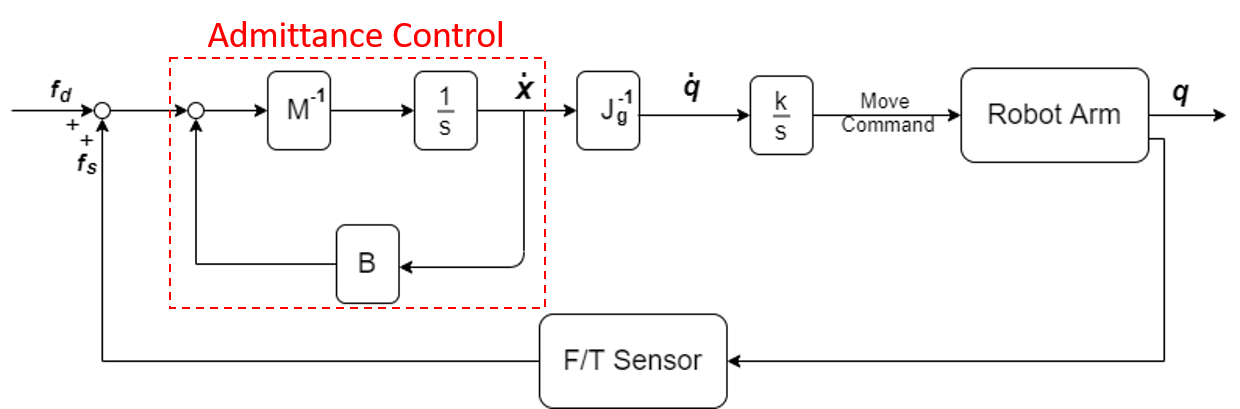
\includegraphics[width=0.9\linewidth]{Images/adm ctrl.png}
\caption{
Control scheme. $\boldsymbol{f_d}$ denotes the desired forces and torques vector. $\boldsymbol{f_s}$ denotes the real value measured by F/T sensor. $\boldsymbol{\dot{x}}$, [$\dot{x}, \dot{y}, \dot{z}, \dot{\theta _x}, \dot{\theta _y}, \dot{\theta _z}$],  denotes the velocity of end effector. $\mathbf{J_g}$ denotes the geometric Jacobian matrix. $\boldsymbol{\dot{\theta }}$, [$\dot{\theta _1}, \dot{\theta _2}, \dot{\theta _3}, \dot{\theta _4}, \dot{\theta _5}, \dot{\theta _6}$], denotes the joints' angular velocities. $\boldsymbol{\theta }$, [$\theta _1, \theta _2, \theta _3, \theta _4, \theta _5, \theta _6 $], denotes the joints' angles. $\mathbf{M}$ is an inertial diagonal matrix, diag($m_1,m_2,\cdots ,m_6$), and $\mathbf{B}$ is a damping diagonal matrix, diag($b_1,b_2,\cdots ,b_6$). $\mathbf{K}$ is a constant gain diagonal matrix, diag($k,k,k,k,k,k$). 
}\label{fig:adm ctrl}
\end{center}
\end{figure}
\hspace*{6mm}Admittance control makes the robot move like a spring-mass-damper system. Forces and torques can be mapped into the movements such as position or velocity. Most importantly, admittance control enables a robot arm to cooperate with humans in a safe work environment \cite{admctrl}. Since Meca500 is an industrial robot arm without admittance control, we subsequently combine the robot arm with the F/T sensor to adopt admittance control. With force and torque feedback, the F/T sensor makes Meca500 be like a collaborative robot arm. a control scheme is proposed and depicted in Figure \ref{fig:adm ctrl}. It's worth noting that in this approach, the admittance control function is triggered by the end effector mounted on the F/T sensor instead of detecting each wrist torque of the robot arm.
\par
A standard equation of admittance control is represented as Equation \ref{eq:adm_mbk}. The values we obtain from the F/T sensor are $\left[f_x, f_y, f_z,\tau _x, \tau _y, \tau _z \right]$, whose forces $ \left[f_x, f_y, f_z\right]$ are related to the translations $ \left[x, y, z\right]$ and torques $ \left[\tau _x, \tau _y, \tau _z\right]$ are related to the axis angle $ \left[\theta _x,\theta _y,\theta _z\right]$. 
\begin{equation}
\label{eq:adm_mbk}
\begin{split}
\begin{bmatrix}
x \\
y \\
z \\
\theta _x \\
\theta _y \\
\theta _z 
\end{bmatrix}
=
\begin{bmatrix}
\frac{1}{m_1s^2+b_1s+k_1}&0  &\cdots  &0 \\ 
0 & \frac{1}{m_2s^2+b_2s+k_2}  & &\vdots \\ 
\vdots& &\ddots  & 0\\ 
0   &\cdots & 0 & \frac{1}{m_6s^2+b_6s+k_6}
\end{bmatrix}
\begin{bmatrix}
f_x \\
f_y \\
f_z \\
\tau _x \\
\tau _y \\
\tau _z 
\end{bmatrix}
\end{split}
\end{equation}
where $[m_1,m_2,\cdots,m_6]$, $[b_1,b_2,\cdots,b_6]$, $[k_1,k_2,\cdots,k_6]$ are inertial, damping and spring parameters of admittance control, 
\subsubsection{Selection of Admittance Control Model}
\hspace*{6mm}In our proposed approach, $\mathbf{K}$ related to spring stiffness is omitted, considering that it's not necessary to bounce such as a spring. Therefore, our system should behave like a mass-damper system. The input is the value measured by F/T sensor and the output is the velocity of end effector shown as 
\begin{equation}
\label{eq:adm_mb}
\begin{split}
\begin{bmatrix}
\dot{x} \\
\dot{y} \\
\dot{z} \\
\dot{\theta _x} \\
\dot{\theta _y }\\
\dot{\theta _z }
\end{bmatrix}
=
\begin{bmatrix}
\frac{1}{m_1s+b_1}&0  &\cdots  &0 \\ 
0 & \frac{1}{m_2s+b_2}  &\ddots  &\vdots \\ 
\vdots&\ddots  &\ddots  & 0\\ 
0   &\cdots & 0 & \frac{1}{m_6s+b_6}
\end{bmatrix}
\begin{bmatrix}
f_x \\
f_y \\
f_z \\
\tau _x \\
\tau _y \\
\tau _z 
\end{bmatrix}
\end{split}
\end{equation}
\subsubsection{Robot Command Decision}
\hspace*{6mm}After determining our admittance control model, we should select a correspondent command to move the robot. However, there are many commands of moving the robot arm, as shown in Table \ref{tab:commands}.
\begin{table}[htbp]
\centering
\tabcolsep=20pt
\caption{Moving commands of Meca500}
\label{tab:commands}
\begin{tabular}{|c|c|l|} 
\hline
\rowcolor{lightgray}Types						&Commands			&Input parameters\\
\cline{1-3}
\multirow{2}{*}{Position}					&MoveJoints			&\noindent $\theta _1, \theta _2 ,\theta _3 ,\theta _4 ,\theta _5 , \theta _6 $\\\cline{2-3}
											&MovePose			&\noindent$x,y,z,\alpha ,\beta ,\gamma $\\
\cline{1-3}
\multirow{2}{*}{Velocity}					&MoveJointsVel		&$\dot{\theta}_1, \dot{\theta}_2, \dot{\theta}_3,\dot{\theta}_4, \dot{\theta}_5 , \dot{\theta}_6 $\\\cline{2-3}
											&MoveLinVelTRF		&$\dot{x},\dot{y},\dot{z},\dot{\theta _x},\dot{\theta _y},\dot{\theta _z}$\\
\hline
\end{tabular}
\end{table}
\par
Position commands is better than velocity commands because Meca500 has a default time-out value to ensure its safety. Even though we could set this value from 0.001 to 2 seconds, Meca500 is still restricted to move with this value. For example, the value of time-out is set $0.1$ sec. While the robot receives a command, the robot move for $0.1$ sec then immediately stops. It's not easy to control via velocity command due to this default property.
\par
Therefore, there are two suitable ways to command robot - MovePose and MoveJoints. Implementation of MovePose $(x,y,z,\alpha ,\beta ,\gamma)$ is easier than MoveJoints because MovePose is considered in tool frame. That means it will move $(x,y,z,\alpha ,\beta ,\gamma)$ based on the current tool frame.  $(x,y,z)$ can be obtained by multiplying an integrator with $(\dot{x},\dot{y},\dot{z})$. As for $(\alpha ,\beta ,\gamma)$, $(\dot{\alpha} ,\dot{\beta} ,\dot{\gamma)}$ can be obtained by multiplying the inverse matrix of analytical jacobian which was mentioned in Equation \ref{eq:jacobian_euler} with $\dot{\theta _x},\dot{\theta _y},\dot{\theta _z}$, and then $(\alpha ,\beta ,\gamma)$ can be obtained by multiplying an integrator with $(\dot{\alpha} ,\dot{\beta} ,\dot{\gamma)}$.
\par
However, considering that the singularity problem is an imperative subject in robotics, we intend to use MoveJoints to set the axes' angles directly. Despite that it's easier to implement admittance control via other commands, the system would touch the singularity point at any time. It undoubtedly exposes patients to danger because of the uncertainty of the system. In our case, we could detect whether it is a singularity or not before commanding the robot. Therefore, position command - MoveJoints and velocity command - MoveJointsVel is our option. 
\par
Finally, we designate MoveJoints $\theta _1, \theta _2 ,\theta _3 ,\theta _4 ,\theta _5 , \theta _6 $ as our main command. Thanks to the property of Jacobian matrix shown in Equation \ref{eq:jg6}, we can transform $\boldsymbol{\dot{x}}$ into $\boldsymbol{\dot{\theta}}$. Then we multiply it an integrator $\frac{1}{\mathrm{s}}$
to obtain $\boldsymbol{\theta}$. Note that, because admittance control is based on frame \{H\}, we should use Equation \ref{eq:jg6} rather than Equation \ref{eq:jg0}. 
\subsubsection{Implementation in Discrete Time}
\hspace*{6mm}To implement it in digital control, the bilinear transformation, also known as Tustin method, is used to control it in discrete time.
\begin{equation}
\label{eq:z_domain eq}
\begin{split}
\frac{v_i(s)}{f_i(s)} &= \frac{1}{m_is+b_i}\\
\Rightarrow 
\frac{v_i(z)}{f_i(z)} &= \frac{t_s \cdot (1+z^{-1})}{(t_s \cdot b_i+2m_i)+(t_s \cdot b_i-2m_i)\cdot z^{-1}}
\end{split}
\end{equation}
and
\begin{equation}
\begin{split}
\frac{\theta_i(s)}{w_i(s)}
				&= \frac{k}{s}\\
\Rightarrow 
\frac{\theta_i(z)}{w_i(z)}
				&= \frac{t_s \cdot k}{2}	
					\frac{1+z^{-1}}{1-z^{-1}}
\end{split}
\end{equation}
where $i = 1,2,\cdots, n$. $(v_1$,$v_2$,$\cdots$,$v_6)$ denote $(\dot{x}$,$\dot{y}$,$\dot{z}$,$\dot{\theta _x}$,$\dot{\theta _y}$,$\dot{\theta _z})$. $(f_1,f_2$,$\cdots,f_6)$ denote $(f_x$,$f_y$,$f_z$,$\tau _x$,$\tau _y$,$\tau _z )$. $(w_1,w_2$,$\cdots,w_6)$ denote $(\dot{\theta _1}, \dot{\theta _2} ,\cdots , \dot{\theta _6} )$. $k$ represents the constant gain. $t_s$ represents the sampling time. $(m_1$,$m_2$,$\cdots$,$m_6)$ and $(b_1$,$b_2$,$\cdots$,$b_6)$ represent inertial and dampoing parameters of admittance control.
\par\noindent
Therefore,
\begin{equation}
\begin{split}
&v_i[\mathrm{k}+1] = \frac{t_s}{t_s \cdot b_i+2m_i}
							\cdot \left(	f_i[\mathrm{k}+1] + f_i[\mathrm{k}]		\right)
						 - \frac{t_s \cdot b_i-2m_i}{t_s \cdot b_i+2m_i}
						 	\cdot v_i[\mathrm{k}]												\\
&\theta_i[\mathrm{k}+1] = \theta_i[\mathrm{k}] + \frac{t_s \cdot k}{2}
												\left( w_i[\mathrm{k}+1] + w_i[\mathrm{k}] \right)
\end{split}
\end{equation}	
\section{Self-Alignment Mode}
\hspace*{6mm}This section aims to adjust the surgical path in real-time. This approach is one of the main contributions in this thesis. A critical technical solution to coordinate transformation of F/T sensor is presented followed by motion planning based on admittance control. 
\subsection*{Coordinate Transformation of F/T sensor}
\label{sec:rfc}
\vspace*{-5mm}
\hspace*{6mm}In "Self-Alignment Mode" DentiBot amend the inserting direction by itself to lower the contact resistance. DentiBot should rotate and move the endodontic file related to the tool-tip frame. Nevertheless, the F/T sensor has its own reference coordinates initially. The F/T sensor originally recognizes its coordinate rather than the tool-tip frame. Namely, the F/T sensor receives unmatched data when the tool contacts an obstacle due to the wrong reference frame \cite{erdogan2014gravity}. Therefore, it is essential to change the reference coordinate of F/T sensor from its original coordinate, frame\{S\}, to tool-tip coordinate, frame\{H\}. We analyze it from two perspectives - reference frame changing and measurement point changing.
\subsubsection{Reference Frame Changing}
\begin{figure}[htbp]
\begin{center}
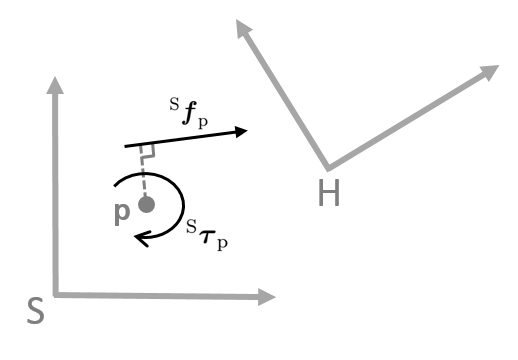
\includegraphics[width=0.6\linewidth]{Images/sensor_comp 1.png}
\caption{
Illustration of changing reference frame from $\{\mathrm{S}\} $ to $\{\mathrm{H}\}$. $\boldsymbol{f}_\mathrm{p}$ and $\boldsymbol{\tau}_\mathrm{p}$ respectively denote a force vector and a torque vector applied at point p and observed from \{S\} and \{H\}.
}\label{fig:sensor_comp1}
\end{center}
\end{figure}
\par\noindent
\hspace{6mm}Figure \ref{fig:sensor_comp1} illustrates a force and a torque applied at point p. The force and torque related to \{S\} and \{H\} are compared and described as   
\begin{equation}
\begin{split}
\begin{bmatrix}
\boldsymbol{f}_\mathrm{p}\\ 
\boldsymbol{\tau}_\mathrm{p}
\end{bmatrix}
_{\{ \mathrm{H}\}}
=
\begin{bmatrix}
_\mathrm{S}^\mathrm{H}\mathbf{R} & \boldsymbol{0}\\ 
\boldsymbol{0} & _\mathrm{S}^\mathrm{H}\mathbf{R}
\end{bmatrix}
\begin{bmatrix}
\boldsymbol{f}_\mathrm{p}\\ 
\boldsymbol{\tau}_\mathrm{p}
\end{bmatrix}
_{\{ \mathrm{S}\}}
\end{split}
\end{equation}
where $\boldsymbol{f}_\mathrm{p}$ and $\boldsymbol{\tau}_\mathrm{p}$ denote the force and the torque applied at point p respectively. $_\mathrm{S}^\mathrm{H}\mathbf{R}$ is the rotation matrix from frame \{S\} to \{H\}.
\subsubsection{Measurement Point Changing}
\begin{figure}[htbp]
\label{fig:sensor_comp2}
\begin{center}
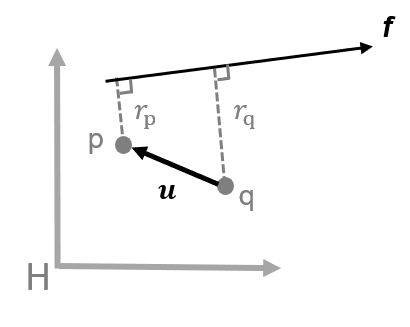
\includegraphics[width=0.65	\linewidth]{Images/sensor_comp 2.png}
\caption{
Illustration of changing measurement point from point p to point q. $\boldsymbol{f}$ denote a force vector applied at frame \{H\} and observed from point p and q. $r_{\mathrm{p}},r_{\mathrm{q}}$ are distances between point p, q and their projections on $\boldsymbol{f}$.
}
\end{center}
\end{figure}
\par\noindent
\hspace{6mm}On the other hand, in Figure \ref{fig:sensor_comp2} the relationship of a force and a torque observed at the same frame but at different points is derived as
\begin{equation}
\begin{split}
\boldsymbol{f}				&= \boldsymbol{f}_\mathrm{p} = \boldsymbol{f}_\mathrm{q}\\
\boldsymbol{\tau}_\mathrm{q} 	&= r_\mathrm{q} \cdot \boldsymbol{f}\\
			 				&= r_\mathrm{p} \cdot \boldsymbol{f}+\boldsymbol{u} \times \boldsymbol{f}_\mathrm{p}\\
			 				&= \boldsymbol{\tau}_\mathrm{p} + \boldsymbol{u}\times \boldsymbol{f}_\mathrm{p}
\end{split}
\end{equation}
\par\noindent
where $\boldsymbol{f}_\mathrm{p}$ and $\boldsymbol{f}_\mathrm{q}$ are respectively represent the same force measured at point p and q. $\boldsymbol{\tau}_\mathrm{p}$ and $\boldsymbol{\tau}_\mathrm{q}$ are respectively represent the same torque measured at point p and q. $\boldsymbol{u}$ denotes the vector from q to p.
\par\noindent
Assume  
\begin{equation*}
\begin{split}
\boldsymbol{u}
=
\begin{bmatrix}
u_1\\
u_2\\
u_3
\end{bmatrix}
\end{split}
\end{equation*}
Then
\begin{equation}
\begin{split}
\boldsymbol{u}\times \boldsymbol{f}_\mathrm{p}
=
\begin{bmatrix}
0		&-u_3		&u_2		\\
u_3		&0			&-u_1		\\
-u_2	&u_1		&0		
\end{bmatrix}
\begin{bmatrix}
f_1\\
f_2\\
f_3
\end{bmatrix}
\end{split}
\end{equation}
\par\noindent
Therefore, 
\begin{equation}
\begin{split}
\begin{bmatrix}
\boldsymbol{f}_\mathrm{q}\\ 
\boldsymbol{\tau}_\mathrm{q}
\end{bmatrix}
_{\{ \mathrm{H}\}}
=
\begin{bmatrix}
\mathbf{I}_{3 \times 3} & \boldsymbol{0}_{3 \times 3}\\ 
\begin{matrix}
0		&-u_3		&u_2		\\
u_3		&0			&-u_1		\\
-u_2	&u_1		&0		
\end{matrix} & \mathbf{I}_{3 \times 3}
\end{bmatrix}
\begin{bmatrix}
\boldsymbol{f}_\mathrm{p}\\ 
\boldsymbol{\tau}_\mathrm{p}
\end{bmatrix}
_{\{ \mathrm{H}\}}
\end{split}
\end{equation}
\par
Finally, reference frame changing and measurement point changing are combined and shown in Equation \ref{eq: ref_sensor}. F/T sensor now can change the reference frame from its original frame \{S\}to the tool-tip frame \{H\}.
\begin{equation}
\label{eq: ref_sensor}
\begin{split}
\begin{bmatrix}
\boldsymbol{f}_\mathrm{q}\\ 
\boldsymbol{\tau}_\mathrm{q}
\end{bmatrix}
_{\{ \mathrm{H}\}}
=
\begin{bmatrix}
\mathbf{I}_{3 \times 3} & \boldsymbol{0}_{3 \times 3}\\ 
\begin{matrix}
0		&-u_3		&u_2		\\
u_3		&0			&-u_1		\\
-u_2	&u_1		&0		
\end{matrix} & \mathbf{I}_{3 \times 3}
\end{bmatrix}
\begin{bmatrix}
_\mathrm{S}^\mathrm{H}\mathbf{R} & \boldsymbol{0}\\ 
\boldsymbol{0} & _\mathrm{S}^\mathrm{H}\mathbf{R}
\end{bmatrix}
\begin{bmatrix}
\boldsymbol{f}_\mathrm{p}\\ 
\boldsymbol{\tau}_\mathrm{p}
\end{bmatrix}
_{\{ \mathrm{S}\}}
\end{split}
\end{equation}
\subsection*{Motion Planning Based on Admittance Control}
\label{sec:motion planning} 
\hspace*{6mm}Here we plan a series of motions to simulate the cleaning procedure of the root canal treatment. Endodontist uses their professional experience to determine how many force to apply and when to reverse the file to release the torque caused by the contact force. Because the root canal resembles a cone. The profundity of the file is larger, then the resultant force composed of contact forces is more significant. Namely, the endodontist will apply more and more pressure in the insertion direction during the surgery. To simulate this series of motions, we could directly command the robot arm to move with the series of actions. However, commanding the robot arm is a dilemma because we have already use admittance control which also commands the robot arm to move. Therefore, to solve the conflict, we continue to utilize admittance control and propose a method based on admittance control to simulate the series of motions. Because we know the tool frame from section \ref{sec:ref_robot}, we can regulate $\boldsymbol{f_d}$ to make the robot move. That means if we want to insert along with the tool direction, we could set [$0$ $0$ $f_z$ $0$ $0$ $0$]. While $f_z$ is larger, the robot moves faster.

\section{Parameter Selection}
\label{sec:affection}
\hspace*{6mm}Because our system is similar to a mass- damper system, we focus on the performance of the velocity $\boldsymbol{\dot{x}}$. The input is the sum of the desired force and sensor values. Therefore, the system could be considered as
\begin{figure}[htbp]
\begin{center}
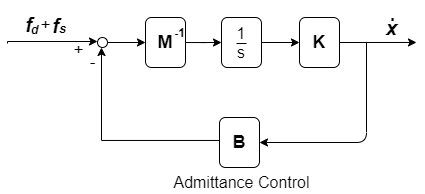
\includegraphics[width=0.55\linewidth]{Images/mass spring.png}
\hspace*{6mm}\end{center}
\caption{
Admittance Control. $\boldsymbol{f_d}$ denotes the desired forces and torques vector. $\boldsymbol{f_s}$ denotes the real value measured by F/T sensor. $\boldsymbol{\dot{x}}$, [$\dot{x}, \dot{y}, \dot{z}, \dot{\theta _x}, \dot{\theta _y}, \dot{\theta _z}$],  denotes the velocity of end effector. $\mathbf{M}$ is an inertial diagonal matrix, diag($m_1,m_2,\cdots ,m_6$), and $\mathbf{B}$ is a damping diagonal matrix, diag($b_1,b_2,\cdots ,b_6$). $\mathbf{K}$ is a constant gain diagonal matrix, diag($k,k,k,k,k,k$). 
}\label{fig:mass spring}
\end{figure}
\par\noindent
It is a first-order control system and its step response is 
\begin{equation}
\begin{split}
\mathcal{L}^{-1} \left[ \frac{1}{s} \cdot \frac{k}{m_is+b_i} \right] 
&= \mathcal{L}^{-1} \left[ \frac{k}{b_i} \left( \frac{1}{s} - \frac{1}{s+\frac{b_i}{m_i}} \right) \right] \\
&= \frac{k}{b_i} \left(1 - e^{- \frac{b_i}{m_i} t}  \right)
\end{split}
\end{equation}
where $i = 1$ to $n$.
\par\noindent
From the above derivation, we can know 
\begin{equation}
\begin{split}
\text{time constant } \tau_i &= \frac{m_i}{b_i}\\
\text{gain} &= \frac{k}{b_i}
\end{split}
\end{equation}
Hence,the transient response can be derived as 
\begin{equation}
\begin{split}
&\text{Rise time} = 2.3\tau_i = \frac{2.3 m_i}{b_i}\\
&\text{Settling time} = 4\tau_i =  \frac{4 m_i}{b_i}\\
\end{split}
\end{equation}
\par
In theory, when $\tau_i$ is larger, the pole is farther from the origin in $\mathrm{s}$ domain, the system is more stable. Besides, when $\tau_i$ is larger, the response speed is faster. Furthermore, when the gain $\frac{k}{b_i}$ is larger, the robot arm moves more. Therefore, we coarse-tune parameter $k$ to adjust the whole gain of the system and determine the mode of the system is "Dragging Mode" or "Self-Alignment Mode". Last but not least, we fine-tune diagonal parameters of $b_i$ separately because the inertial and spring properties of each axis are discrepant. 
\par
In practice, we implement it in discrete time. From Equation \ref{eq:z_domain eq}, we can further derive the final value in discrete time shown as 
\begin{equation}
\begin{split}
\text{gain} = \lim_{z \to 1} (z-1)\cdot \frac{t_s \cdot k(z+1)}{(t_s \cdot b_i+2m_i)z+t_s \cdot b_i-2m_i}\cdot \frac{1}{\frac{2}{t_s}\frac{z-1}{z+1}} = \frac{k\cdot t_s}{b_i}
\end{split}
\end{equation}
Compared to the gain in continuous time, the sampling time in discrete time also affect the gain. Because the sampling time we set is $0.002$s, we set $(m_i : b_i = 1 : 500)$  to make $(\tau _i = \frac{m_i}{b_i} = 0.002)$, then the system will rise up to $98\%$ after $0.004$ second. Further, we can alter $k$ to easily regulate the gain. It is worth noting that the rotation along with Z-axis driven by the robot arm should be deactivated in "Self-Alignment Mode" because the file rotation is driven by the motor. If the rotation along with z-axis is on duty and the file is drilling, the robot arm would rotate along with Z-axis in opposite direction. Hence, $b_6$ is set a infinite value to deactivate the rotation along with Z-axis. Detailed parameters setting of admittance control with "Dragging Mode" and "Self-Alignment Mode" are shown in Table \ref{tab: para_adm}.
\begin{table}[htbp]
\centering
\caption{Parameters setting of Admittance control.}
\label{tab: para_adm}
\begin{tabular}{ccc} 
\hline \hline
Parameter	&Dragging Mode		&Self-Alignment Mode	\\
\hline
k			&$1500$				&$500$				\\
$b_1$		&$80$				&$80$					\\
$b_2$		&$80$				&$80$					\\
$b_3$		&$80$				&$80$					\\
$b_4$		&$160$				&$80$					\\
$b_5$		&$160$				&$80$					\\
$b_6$		&$160$				&$\infty$					\\
%$m_1$		&$0.004$			&$0.012$				\\
%$m_2$		&$0.004$			&$0.006$				\\
%$m_3$		&$0.004$			&$0.011$				\\
%$m_4$		&$0.008$			&$0.017$				\\
%$m_5$		&$0.008$			&$0.04$					\\
%$m_6$		&$0.008$			&$0.018$		
\hline	
&$\mathbf{K} = \text{diag}(k,k,k,k,k,k),$ &$\mathbf{B} = \text{diag}(b_1,b_2,b_3,b_4,b_5,b_6)$\\
\hline\hline	
\end{tabular}
\end{table}
\begin{figure}[htbp]
\begin{center}
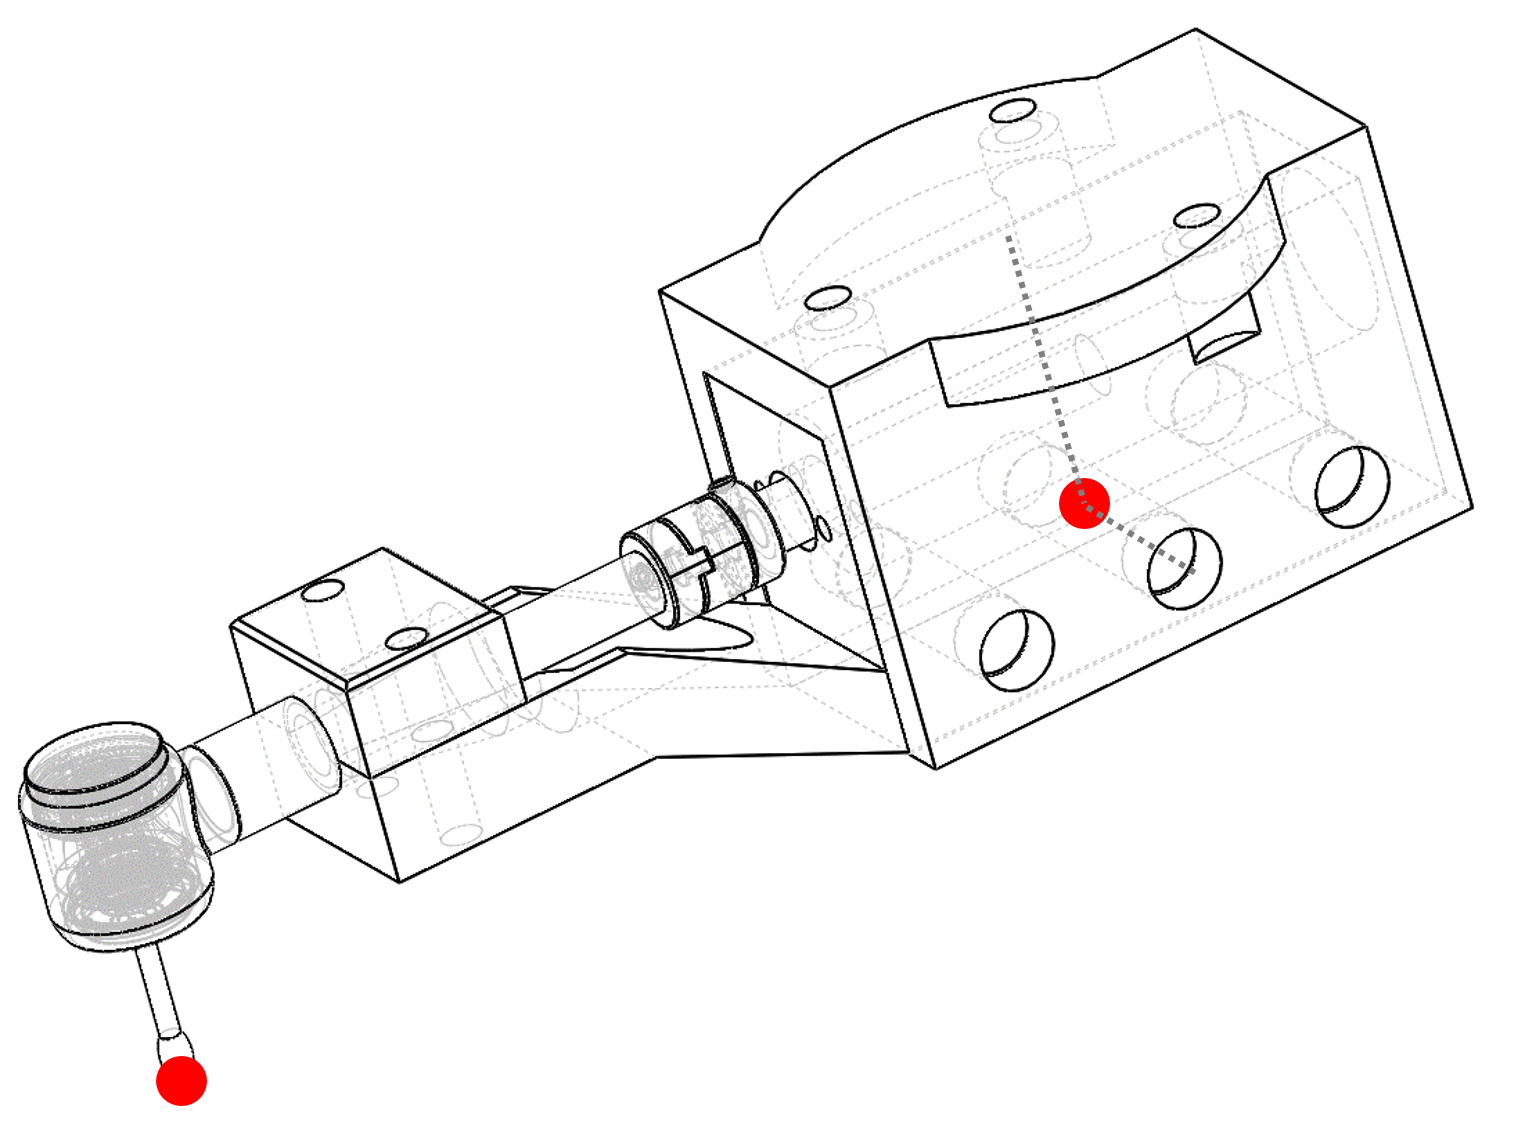
\includegraphics[width=0.7\linewidth]{Images/holding_gesture.png}
\caption{
Reference point A in Dragging Mode. Reference point B and holding points $G_1,G_2$ in Self-Alignment Mode.
}\label{fig:holding gesture}
\end{center}
\end{figure}
\par
Note that we change the different sensor frames in "Dragging Mode" and "Self-Alignment Mode". As shown in Figure \ref{fig:holding gesture}, Point A and B are two origins of the sensor frame. In "Dragging Mode", we transform the sensor frame to the point A, and the operator can hold the point $\mathrm{G_1}$ and $\mathrm{G_2}$ to move the entire handpiece. On the other hand, in "Self-Alignment Mode" we set  the point B as the new sensor frame because we focus on forces and torques the file bears. Due to different level arms, the forces we apply in each axis will be different. There are same level arms ($\overline{\mathrm{AO}}$ and $\overline{\mathrm{OG_2}}$ both are $13.2$ mm) if we set the point A as the sensor frame and grasp $\mathrm{G_1}$ and $\mathrm{G_2}$ to move the entire handpiec. Therefore, to provide users a good experience, we should regulate parameters of $\mathbf{B}$ in "Dragging mode" with suitable values. With these values, the users can smoothly move the robot arm to the desired position and orientation. We set the first three variables relative to the linear velocity as the same values. Besides, We set the last three variables relative to the angular velocity as the other same values.
